% Review 2 deck -- compile with pdflatex (run twice). Self-contained: no other files needed.
\documentclass[aspectratio=169,11pt]{beamer}
% ---------------- theme (identical in review1.tex and review2.tex) ----------------
\usepackage[T1]{fontenc}
\usepackage{lmodern}
\usepackage{amsmath}
\usepackage{booktabs}
\usepackage{tabularx}
\usepackage{array}
\usepackage{listings}
\usepackage{tikz}
\usetikzlibrary{arrows.meta,positioning,calc,fit,backgrounds,shapes.geometric}

% ---------------------------------------------------------------- colours
\definecolor{paper}{HTML}{F3EDE2}
\definecolor{card}{HTML}{FBF8F2}
\definecolor{ink}{HTML}{1F1B16}
\definecolor{muted}{HTML}{6B6358}
\definecolor{rulec}{HTML}{CFC5B4}
\definecolor{accent}{HTML}{C8421B}
\definecolor{eventc}{HTML}{B7791F}
\definecolor{resc}{HTML}{1D5E5B}
\definecolor{volc}{HTML}{274B8F}
\definecolor{budc}{HTML}{5F6D1C}

\setbeamercolor{background canvas}{bg=paper}
\setbeamercolor{normal text}{fg=ink}
\setbeamercolor{structure}{fg=accent}
\setbeamercolor{alerted text}{fg=accent}
\setbeamercolor{itemize item}{fg=accent}
\setbeamercolor{itemize subitem}{fg=muted}
\setbeamertemplate{itemize item}{\small\raise1.2pt\hbox{\textbullet}}
\setbeamertemplate{itemize subitem}{\scriptsize\raise1pt\hbox{--}}
\setbeamertemplate{navigation symbols}{}

\setbeamertemplate{frametitle}{%
  \vspace{3pt}%
  {\color{accent}\scriptsize\ttfamily\bfseries \insertsubsection}\par
  {\color{ink}\Large\bfseries \insertframetitle}\par
  \vspace{2pt}{\color{ink}\rule{\textwidth}{0.6pt}}%
}
\setbeamertemplate{footline}{%
  \hspace{1.2em}{\color{muted}\tiny\ttfamily \footlinetext}\hfill
  {\color{accent}\tiny\ttfamily\bfseries \insertframenumber\,/\,\inserttotalframenumber}\hspace{1.2em}\vspace{8pt}%
}

% ---------------------------------------------------------------- helpers
\newcommand{\rs}{Rs.\,}
% \card{colour}{LABEL}{body}
\newcommand{\card}[3]{%
  \begin{tikzpicture}
    \node[draw=rulec, fill=card, line width=0.5pt, text width=\linewidth-14pt, inner sep=6pt, align=left] (c) {%
      {\color{#1}\scriptsize\ttfamily\bfseries #2}\par\vspace{2pt}\footnotesize #3};
    \draw[#1, line width=3pt] (c.north west) -- (c.north east);
  \end{tikzpicture}}

\tikzset{
  agent/.style={draw=#1, fill=card, line width=0.8pt, rounded corners=2pt, minimum height=9mm,
                text width=24mm, align=center, font=\scriptsize\bfseries},
  topbar/.style={draw=#1, line width=3pt},
  msg/.style={-{Stealth[length=2mm]}, line width=0.7pt, color=#1},
  lbl/.style={font=\tiny\ttfamily, fill=paper, inner sep=1pt},
  layer/.style={draw=#1, fill=card, line width=0.7pt, minimum width=128mm, minimum height=9mm,
                align=left, text width=124mm, font=\scriptsize},
  box/.style={draw=#1, fill=card, line width=0.7pt, rounded corners=2pt,
              text width=30mm, minimum height=9mm, align=center, font=\scriptsize},
}

\lstset{basicstyle=\ttfamily\tiny, keywordstyle=\color{accent}\bfseries, commentstyle=\color{muted}\itshape,
        stringstyle=\color{resc}, backgroundcolor=\color{card}, frame=single, rulecolor=\color{rulec},
        framesep=4pt, xleftmargin=4pt, xrightmargin=4pt, columns=fullflexible, keepspaces=true,
        showstringspaces=false, language=Python}

% ---------------------------------------------------------------- title page
\setbeamertemplate{title page}{%
  \begin{tikzpicture}[remember picture, overlay]
    \fill[ink] (current page.north west) rectangle ([yshift=-7mm]current page.north east);
    \node[anchor=west, text=paper, font=\tiny\ttfamily\bfseries] at ([xshift=8mm,yshift=-3.5mm]current page.north west)
      {CAMPUS FEST '26 \quad RESOURCE DESK \quad \reviewlabel};
  \end{tikzpicture}
  \vspace{10mm}
  {\color{accent}\footnotesize\ttfamily\bfseries \insertsubtitle}\par\vspace{4pt}
  {\color{ink}\fontsize{26}{28}\selectfont\bfseries \inserttitle}\par\vspace{10pt}
  {\color{ink}\rule{0.55\textwidth}{0.8pt}}\par\vspace{8pt}
  {\small \insertauthor}\par\vspace{6pt}
  {\footnotesize\color{muted} \insertinstitute}\par\vspace{4pt}
  {\footnotesize\color{muted}\ttfamily \insertdate}
}

\newcommand{\reviewlabel}{REVIEW 2}
\newcommand{\footlinetext}{Campus Fest Resource Allocation \textbullet{} Review 2}

\title{Campus Fest Resource Allocation System}
\subtitle{IMPLEMENTATION, DEMO \& TESTING \textbullet{} REVIEW 2}
\author{Member 1 (Reg.\ No.) \quad Member 2 (Reg.\ No.) \quad Member 3 (Reg.\ No.) \quad Member 4 (Reg.\ No.)}
\institute{Foundations of AI \textbullet{} Guide: Prof.\ \rule{25mm}{0.4pt} \textbullet{} Department of CSE, Your College}
\date{\today}

\begin{document}

% ------------------------------------------------------------------ 1
\begin{frame}[plain]
  \titlepage
\end{frame}

% ------------------------------------------------------------------ 2
\subsection{01 \textbullet{} IMPLEMENTATION}
\begin{frame}{Implementation architecture}
  \centering
  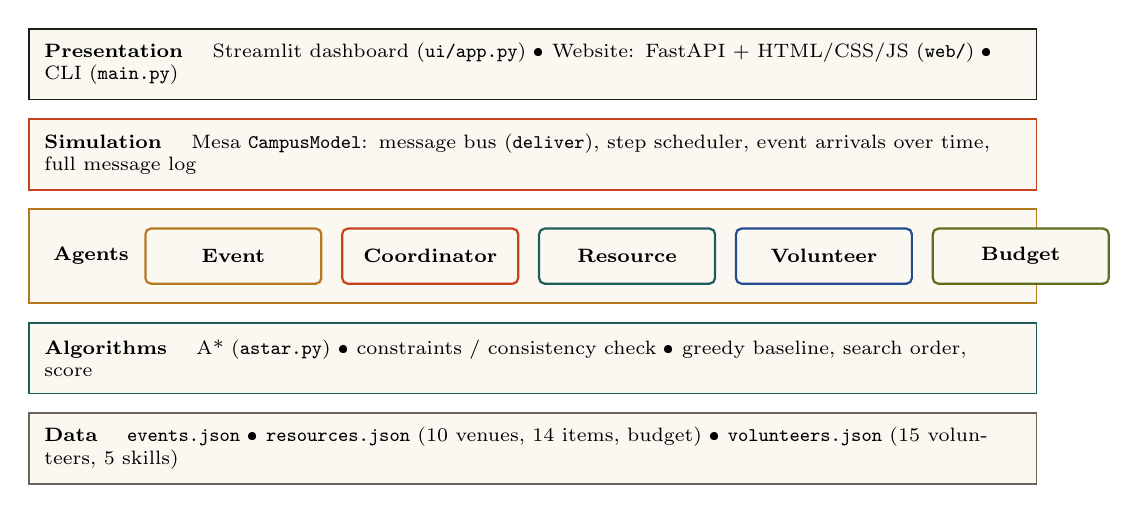
\begin{tikzpicture}[node distance=2.2mm]
    \node[layer=ink] (ui) {\textbf{Presentation} \quad Streamlit dashboard (\texttt{ui/app.py}) \textbullet{}
       Website: FastAPI + HTML/CSS/JS (\texttt{web/}) \textbullet{} CLI (\texttt{main.py})};
    \node[layer=accent, below=of ui] (sim) {\textbf{Simulation} \quad Mesa \texttt{CampusModel}: message bus
       (\texttt{deliver}), step scheduler, event arrivals over time, full message log};
    \node[layer=eventc, below=of sim, minimum height=12mm] (ag) {};
    \node[anchor=west, font=\scriptsize\bfseries] at ([xshift=2mm]ag.west) {Agents};
    \foreach \n/\col/\x in {Event/eventc/-38, Coordinator/accent/-13, Resource/resc/12, Volunteer/volc/37, Budget/budc/62} {
      \node[agent=\col, text width=20mm, minimum height=7mm] at ([xshift=\x mm]ag.center) {\n};
    }
    \node[layer=resc, below=of ag] (alg) {\textbf{Algorithms} \quad A* (\texttt{astar.py}) \textbullet{}
       constraints / consistency check \textbullet{} greedy baseline, search order, score};
    \node[layer=muted, below=of alg] (data) {\textbf{Data} \quad \texttt{events.json} \textbullet{}
       \texttt{resources.json} (10 venues, 14 items, budget) \textbullet{} \texttt{volunteers.json} (15 volunteers, 5 skills)};
  \end{tikzpicture}
\end{frame}

% ------------------------------------------------------------------ 3
\begin{frame}{Technology stack}
  \scriptsize
  \begin{tabularx}{\textwidth}{@{}l l X@{}}
    \toprule
    \textbf{Layer} & \textbf{Technology} & \textbf{Why} \\
    \midrule
    Language        & Python 3           & Readable, rich ecosystem for AI and web \\
    Agent framework & Mesa 3             & Standard agent-based modelling: \texttt{Model}, \texttt{Agent}, agent sets, stepping \\
    Search          & \texttt{heapq} (stdlib) & Priority queue for A*; no extra dependency \\
    Dashboard       & Streamlit + Altair + pandas & Live fest board, booking form, scenario explorer \\
    Website         & FastAPI + Pydantic + vanilla JS & Real agents behind a small REST API; input validation at the boundary \\
    Testing         & pytest            & 21 automated tests: agents, allocation, conflicts \\
    Data            & JSON              & Campus catalogue editable without touching code \\
    \bottomrule
  \end{tabularx}
  \vspace{8pt}

  \card{accent}{DESIGN CHOICE}{Deterministic rule-based agents, not LLM agents: the same input always gives the
    same allocation, so every decision can be explained, tested and defended.}
\end{frame}

% ------------------------------------------------------------------ 4
\begin{frame}[fragile]{Agent implementation}
  \begin{columns}[T]
    \begin{column}{0.53\textwidth}
\begin{lstlisting}
class CampusAgent(mesa.Agent):
    """Owns private state; talks only by messages."""
    def send(self, receiver, performative, text="", **content):
        return self.model.deliver(
            Message(self.name, receiver, performative, content, text))

    def receive(self, msg):
        handler = getattr(self, "on_" + msg.performative.lower(), None)
        if handler is None:
            return self.reply(msg, "NOT_UNDERSTOOD")
        return handler(msg)

class BudgetAgent(CampusAgent):
    def on_commit(self, msg):
        if msg.content["cost"] > self.remaining:
            return self.reply(msg, "REFUSE")
        self.ledger[msg.content["event"]] = msg.content["cost"]
        return self.reply(msg, "COMMITTED")
\end{lstlisting}
    \end{column}
    \begin{column}{0.44\textwidth}
      \scriptsize
      \begin{itemize}\setlength\itemsep{2pt}
        \item \textcolor{eventc}{\textbf{EventAgent}}: \texttt{step} (submit on arrival), \texttt{on\_evaluate}, \texttt{on\_propose}
        \item \textcolor{resc}{\textbf{ResourceAgent}}: \texttt{on\_query}, \texttt{on\_commit}, \texttt{on\_release}; calendar of bookings
        \item \textcolor{volc}{\textbf{VolunteerAgent}}: per-window offers, borrowing from the general pool
        \item \textcolor{budc}{\textbf{BudgetAgent}}: \texttt{on\_quote}, \texttt{on\_balance}, \texttt{on\_commit}
        \item \textcolor{accent}{\textbf{CoordinatorAgent}}: \texttt{gather}, \texttt{preempt}, \texttt{plan} (A*), \texttt{commit}
      \end{itemize}
      \vspace{4pt}
      \card{accent}{KEY POINT}{The Coordinator has no reference to any calendar or ledger. Every fact it uses
        arrives in a reply message.}
    \end{column}
  \end{columns}
\end{frame}

% ------------------------------------------------------------------ 5
\begin{frame}{Agent communication protocol}
  \centering
  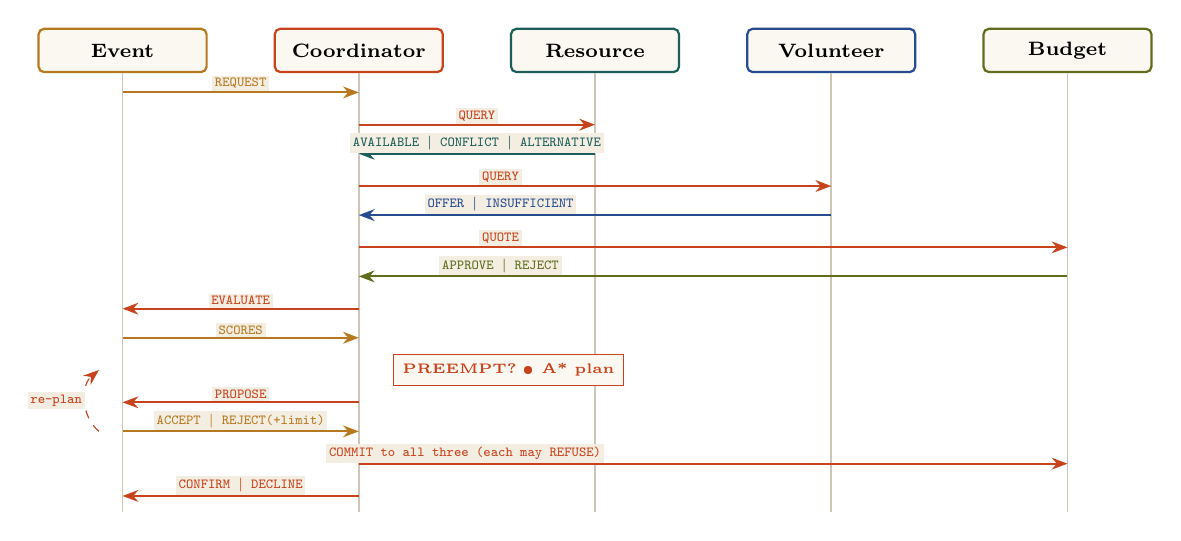
\begin{tikzpicture}[x=10mm, y=4.1mm]
    \foreach \x/\n/\col in {0/Event/eventc, 3/Coordinator/accent, 6/Resource/resc, 9/Volunteer/volc, 12/Budget/budc} {
      \node[agent=\col, text width=19mm, minimum height=5.5mm] at (\x,0) {\n};
      \draw[rulec, line width=0.6pt] (\x,-0.7) -- (\x,-14.3);
    }
    \draw[msg=eventc] (0,-1.3)  -- node[lbl, above] {REQUEST} (3,-1.3);
    \draw[msg=accent] (3,-2.3)  -- node[lbl, above] {QUERY} (6,-2.3);
    \draw[msg=resc]   (6,-3.2)  -- node[lbl, above] {AVAILABLE $|$ CONFLICT $|$ ALTERNATIVE} (3,-3.2);
    \draw[msg=accent] (3,-4.2)  -- node[lbl, above, pos=0.3] {QUERY} (9,-4.2);
    \draw[msg=volc]   (9,-5.1)  -- node[lbl, above, pos=0.7] {OFFER $|$ INSUFFICIENT} (3,-5.1);
    \draw[msg=accent] (3,-6.1)  -- node[lbl, above, pos=0.2] {QUOTE} (12,-6.1);
    \draw[msg=budc]   (12,-7)   -- node[lbl, above, pos=0.8] {APPROVE $|$ REJECT} (3,-7);
    \draw[msg=accent] (3,-8)    -- node[lbl, above] {EVALUATE} (0,-8);
    \draw[msg=eventc] (0,-8.9)  -- node[lbl, above] {SCORES} (3,-8.9);
    \node[draw=accent, fill=card, font=\tiny\bfseries, text=accent] at (4.9,-9.9) {PREEMPT? \textbullet{} A* plan};
    \draw[msg=accent] (3,-10.9) -- node[lbl, above] {PROPOSE} (0,-10.9);
    \draw[msg=eventc] (0,-11.8) -- node[lbl, above] {ACCEPT $|$ REJECT(+limit)} (3,-11.8);
    \draw[msg=accent] (3,-12.8) -- node[lbl, above, pos=0.15] {COMMIT to all three (each may REFUSE)} (12,-12.8);
    \draw[msg=accent] (3,-13.8) -- node[lbl, above] {CONFIRM $|$ DECLINE} (0,-13.8);
    \draw[accent, dashed, -{Stealth[length=2mm]}] (-0.3,-11.8) to[bend left=50] node[lbl, left, text=accent] {re-plan} (-0.3,-9.9);
  \end{tikzpicture}
\end{frame}

% ------------------------------------------------------------------ 6
\subsection{02 \textbullet{} ALGORITHM}
\begin{frame}[fragile]{Allocation algorithm: A* over partial plans}
  \begin{columns}[T]
    \begin{column}{0.58\textwidth}
\begin{lstlisting}
def astar(events, options, reject_cost, check):
    h = suffix sums of min(best option, reject)  # admissible
    frontier = [(h[0], 0, 0.0, ())]              # f, depth, g, path
    while frontier:
        f, i, g, path = heappop(frontier)
        if i == len(events):
            return dict(zip(events, path))       # optimal plan
        e = events[i]
        assigned = [o for o in path if o]
        for o in options[e]:                     # ALLOCATE
            if check(o, assigned) is None:       # constraints
                push(g + o.penalty + h[i+1], i+1, path + (o,))
        push(g + reject_cost[e] + h[i+1], i+1, path + (None,))
\end{lstlisting}
    \end{column}
    \begin{column}{0.39\textwidth}
      \card{accent}{CONSTRAINT CHECK}{%
        \begin{itemize}\setlength\itemsep{0pt}
          \item same venue + overlap $\Rightarrow$ clash
          \item pooled demand $\le$ free count reported by agents
          \item running cost $\le$ budget left
          \item dependencies finish first
        \end{itemize}}
      \vspace{4pt}
      \card{resc}{SAFETY NET}{Expansion cap of 200{,}000 states, then greedy fallback.
        The full-day scenario (8 events) solves instantly.}
    \end{column}
  \end{columns}
\end{frame}

% ------------------------------------------------------------------ 7
\begin{frame}{Negotiation loop inside the Coordinator}
  \centering
  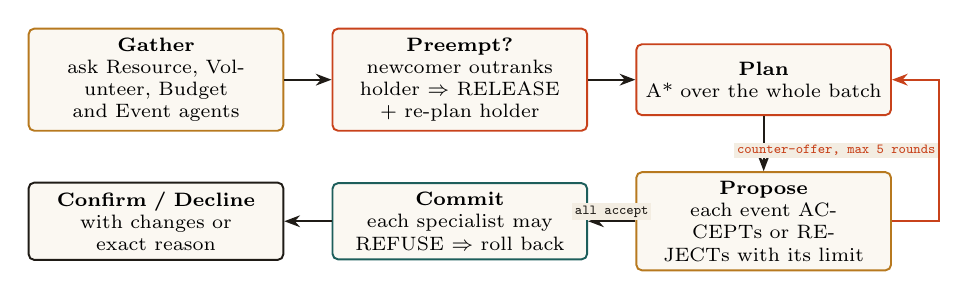
\begin{tikzpicture}[node distance=4mm and 6mm]
    \node[box=eventc] (g) {\textbf{Gather}\\ask Resource, Volunteer, Budget and Event agents};
    \node[box=accent, right=of g] (p) {\textbf{Preempt?}\\newcomer outranks holder $\Rightarrow$ RELEASE + re-plan holder};
    \node[box=accent, right=of p] (a) {\textbf{Plan}\\A* over the whole batch};
    \node[box=eventc, below=7mm of a] (pr) {\textbf{Propose}\\each event ACCEPTs or REJECTs with its limit};
    \node[box=resc, left=of pr] (c) {\textbf{Commit}\\each specialist may REFUSE $\Rightarrow$ roll back};
    \node[box=ink, left=of c] (r) {\textbf{Confirm / Decline}\\with changes or exact reason};
    \draw[msg=ink] (g) -- (p); \draw[msg=ink] (p) -- (a); \draw[msg=ink] (a) -- (pr);
    \draw[msg=ink] (pr) -- node[lbl, above] {all accept} (c); \draw[msg=ink] (c) -- (r);
    \draw[msg=accent] (pr.east) -- ++(6mm,0) |- node[lbl, left, pos=0.25] {counter-offer, max 5 rounds} (a.east);
  \end{tikzpicture}
  \vspace{4pt}

  \footnotesize
  \begin{columns}[T]
    \begin{column}{0.48\textwidth}
      \card{accent}{PRIORITY RULE}{Step cost $= p \times d$; reject $= 25p$. A higher-priority newcomer may
        preempt a lower-priority booking, which is re-planned, not dropped.}
    \end{column}
    \begin{column}{0.48\textwidth}
      \card{volc}{PRIVATE INFORMATION}{An event's minimum acceptable volunteer ratio is revealed only
        in its REJECT. The Coordinator learns it and re-plans.}
    \end{column}
  \end{columns}
\end{frame}

% ------------------------------------------------------------------ 8
\subsection{03 \textbullet{} LIVE DEMO}
\begin{frame}[fragile]{Live demo}
  \begin{columns}[T]
    \begin{column}{0.48\textwidth}
      \card{accent}{WEBSITE: THE FEST DESK}{%
\texttt{python -m uvicorn web.server:app}\\
        \texttt{http://127.0.0.1:8000}\\[3pt]
        Today's programme (happening now / upcoming / finished / not booked), free-slot board,
        booking slip, animated agent conversation, all review scenarios
        (deep link: \texttt{/\#scenario-5}).}
    \end{column}
    \begin{column}{0.48\textwidth}
      \card{resc}{STREAMLIT DASHBOARD}{%
        \texttt{python -m streamlit run ui/app.py}\\[3pt]
        Live fest desk: all events with status, venue $\times$ hour free board, free equipment and volunteers,
        ``Book your event'' form. Review mode: editable scenario JSON, Gantt chart, A* vs greedy.}
    \end{column}
  \end{columns}
  \vspace{4pt}
  \card{eventc}{DEMO SCRIPT (5 MIN)}{%
    \textbf{1} Fest board \quad \textbf{2} Book a p5 keynote in Seminar-Hall at 10:00 (preempts Art Exhibition)
    \quad \textbf{3} Scenarios 2--6 in the theatre \quad \textbf{4} Scenario 8: A* vs greedy}
\end{frame}

% ------------------------------------------------------------------ 9
\begin{frame}{Demo scenarios 1--5: actual system output}
  \scriptsize
  \begin{tabularx}{\textwidth}{@{}l X X r@{}}
    \toprule
    \textbf{Scenario} & \textbf{Input} & \textbf{What the agents did} & \textbf{Score} \\
    \midrule
    1 Normal        & Hackathon, 120 people, Lab-1, projector, 10--13 & Lab-1 10--13, Projector-1, V01 V04 V07, \rs 5{,}500 & 0.854 \\
    2 Resource conflict & Hackathon (p5) and Robotics (p4) both want Lab-1 & CONFLICT noted; Hackathon keeps Lab-1, Robotics $\rightarrow$ Lab-2 & 0.857 \\
    3 Budget conflict   & \rs 45{,}000 of \rs 50{,}000 spent; Main-Stage costs \rs 15{,}000 & Budget REJECT; cheaper Open-Air-Stage at \rs 4{,}000 & 0.854 \\
    4 Volunteer shortage & 5 technical needed, 3 exist & INSUFFICIENT; 3 + 1 borrowed general = 80\,\% (event accepts $\ge$ 60\,\%) & 0.854 \\
    5 High priority     & Poetry Slam (p2) holds Seminar-Hall; Keynote (p5) arrives & PREEMPT; Keynote $\rightarrow$ Seminar-Hall, Poetry Slam $\rightarrow$ Auditorium & 0.854 \\
    \bottomrule
  \end{tabularx}
  \vspace{6pt}
  {\footnotesize\color{muted} Every row is produced by the running system (\texttt{python main.py}); scores use the PEAS formula.}
\end{frame}

\begin{frame}{Scenarios 6--9: negotiation, rescheduling, search, full day}
  \scriptsize
  \begin{tabularx}{\textwidth}{@{}l X X r@{}}
    \toprule
    \textbf{Scenario} & \textbf{Input} & \textbf{What the agents did} & \textbf{Score} \\
    \midrule
    6 Counter-offer     & AI Workshop offered 50\,\% volunteers, needs 90\,\% & REJECT with limit; re-plan: 13--15 with 100\,\% & 0.845 \\
    7 Labs full         & 4 lab sessions 10--13, 3 labs & Flexible session rescheduled to 13--16 & 0.858 \\
    8 A* vs greedy      & Budget \rs 16{,}000, two events & A* schedules both; greedy rejects one & 0.855 vs 0.465 \\
    9 Full fest day     & 8 events incl.\ a dependency & 8/8 booked, 0 double bookings, 148 messages & 0.881 \\
    \bottomrule
  \end{tabularx}
\end{frame}

% ------------------------------------------------------------------ 10
\subsection{04 \textbullet{} TESTING}
\begin{frame}{Testing scenarios (pytest)}
  \scriptsize
  \begin{tabularx}{\textwidth}{@{}l l X l@{}}
    \toprule
    \textbf{Test} & \textbf{Input} & \textbf{Expected} & \textbf{Result} \\
    \midrule
    T1 & Available venue            & Allocate Lab-1 10--13 with equipment and volunteers         & \textcolor{resc}{\textbf{PASS}} \\
    T2 & Same venue and time        & Conflict detected; lower priority moved to Lab-2              & \textcolor{resc}{\textbf{PASS}} \\
    T3 & Insufficient budget        & Budget REJECT, then cheaper alternative within \rs 5{,}000    & \textcolor{resc}{\textbf{PASS}} \\
    T4 & Volunteer shortage         & Reduced allocation with a borrowed general volunteer          & \textcolor{resc}{\textbf{PASS}} \\
    T5 & Multiple simultaneous events & All 8 coordinated, dependencies respected, no double booking & \textcolor{resc}{\textbf{PASS}} \\
    T6 & Invalid resource / time    & ERROR from Resource agent / \texttt{ValueError}               & \textcolor{resc}{\textbf{PASS}} \\
    T7 & Zero budget                & Reject                                                        & \textcolor{resc}{\textbf{PASS}} \\
    T8 & Fully occupied labs        & Flexible event rescheduled                                    & \textcolor{resc}{\textbf{PASS}} \\
    +  & Priority-5 arrives later   & Preempt, displaced event gets an alternative                  & \textcolor{resc}{\textbf{PASS}} \\
    +  & Event rejects an offer     & Coordinator re-plans with the revealed limit                  & \textcolor{resc}{\textbf{PASS}} \\
    +  & Dependency rejected        & Dependent event rejected with reason                          & \textcolor{resc}{\textbf{PASS}} \\
    \bottomrule
  \end{tabularx}
\end{frame}

% ------------------------------------------------------------------ 11
\begin{frame}{Test results}
  \begin{columns}[c]
    \begin{column}{0.44\textwidth}
      \centering
      {\fontsize{44}{46}\selectfont\bfseries\color{resc} 21 / 21}\par
      {\footnotesize\ttfamily\color{muted} tests passed in 1.7 s}\par\vspace{10pt}
      \footnotesize
      \begin{tabular}{@{}lr@{}}
        \toprule
        \texttt{test\_agents.py}     & 6 \\
        \texttt{test\_allocation.py} & 6 \\
        \texttt{test\_conflicts.py}  & 9 \\
        \bottomrule
      \end{tabular}
    \end{column}
    \begin{column}{0.52\textwidth}
      \card{accent}{A* VS GREEDY (SCENARIO 8)}{%
        
\begin{tikzpicture}[x=40mm, y=5mm]
          \foreach \y/\n/\v/\col in {0/A*/0.855/resc, 1/Greedy/0.465/muted} {
            \node[anchor=east, font=\scriptsize\bfseries] at (0,-\y) {\n};
            \fill[\col] (0.02,-\y-0.35) rectangle (\v,-\y+0.35);
            \node[anchor=west, font=\scriptsize\ttfamily] at (\v,-\y) {\v};
          }
        \end{tikzpicture}\\[3pt]
        Greedy gives the Auditorium to the keynote, spends the budget, and rejects the workshop.
        A* moves the keynote to Seminar-Hall and fits both.}
      \vspace{4pt}
      \card{resc}{PROPERTIES CHECKED ON EVERY SCENARIO}{0 double bookings \textbullet{} A* never scores below greedy
        \textbullet{} agents interact only through messages}
    \end{column}
  \end{columns}
\end{frame}

% ------------------------------------------------------------------ 12
\subsection{05 \textbullet{} CODE \& SCALABILITY}
\begin{frame}[fragile]{Code structure}
  \begin{columns}[T]
    \begin{column}{0.5\textwidth}
\begin{lstlisting}[language={}, backgroundcolor=\color{card}]
campus-fest-resource-allocation/
  agents/       base.py (messages)
                event_agent.py  resource_agent.py
                volunteer_agent.py  budget_agent.py
                coordinator_agent.py
  algorithms/   astar.py  constraints.py
                allocation.py (greedy, score)
  environment/  campus.py (Mesa model, bus)
                resources.py  scenarios.py
  data/         events.json  resources.json
                volunteers.json
  tests/        test_agents.py  test_allocation.py
                test_conflicts.py
  ui/app.py     Streamlit dashboard
  web/          server.py (FastAPI) + static/
  main.py       CLI demo
\end{lstlisting}
    \end{column}
    \begin{column}{0.46\textwidth}
      \card{accent}{SEPARATION OF CONCERNS}{%
        \begin{itemize}\setlength\itemsep{0pt}
          \item Agents never import each other: only messages
          \item Algorithms are pure functions, tested alone
          \item Campus data lives in JSON, not in code
          \item Two front-ends share one model
        \end{itemize}}
      \vspace{4pt}
      \card{resc}{ADDING A NEW AGENT}{Subclass \texttt{CampusAgent}, add \texttt{on\_<performative>} handlers,
        register it in \texttt{CampusModel}. Nothing else changes.}
    \end{column}
  \end{columns}
\end{frame}

% ------------------------------------------------------------------ 13
\begin{frame}{Future scalability}
  \begin{columns}[T]
    \begin{column}{0.48\textwidth}
      \card{accent}{MORE SCALE}{%
        \begin{itemize}\setlength\itemsep{0pt}
          \item Multi-day fests: add a day to every slot
          \item Beam search or weighted A* when events grow beyond hundreds
          \item Persistent bookings in a database
        \end{itemize}}
    \end{column}
    \begin{column}{0.48\textwidth}
      \card{resc}{MORE INTELLIGENCE}{%
        \begin{itemize}\setlength\itemsep{0pt}
          \item Auction or Contract-Net bidding between event agents
          \item Learn deviation weights from organiser feedback
          \item Uncertainty: no-shows, overruns, weather for open-air venues
        \end{itemize}}
    \end{column}
  \end{columns}
  \vspace{4pt}
  \card{volc}{NEW AGENT TYPES THAT PLUG IN}{Transport agent (vehicles and routes) \textbullet{}
    Catering agent (food stalls and menus) \textbullet{} Security agent (crowd limits per venue)}
\end{frame}

% ------------------------------------------------------------------ 14
\begin{frame}[plain]
  \vfill
  \centering
  {\color{accent}\ttfamily\small THANK YOU}\par\vspace{6pt}
  {\fontsize{30}{32}\selectfont\bfseries Questions?}\par\vspace{10pt}
  {\color{ink}\rule{0.3\textwidth}{0.8pt}}\par\vspace{8pt}
  {\footnotesize\color{muted} 5 agents \textbullet{} 9 scenarios \textbullet{} 21 tests passed \textbullet{} 0 double bookings}
  \vfill
\end{frame}

\end{document}
